\label{documentation-generation}
When invoked with the {\tt $-$focalize-doc} option, the command
{\focalizec} generates an extra file (with the ``.fcd'' suffix)
containing ``documentation'' information extracted from the compiled
source file.

This information describes the different elements found in the source
file (species, collections, methods, toplevel definitions, type
definitions) with various annotations like type,
definition/inheritance locations. It also contains the special comments
previously called {\bf annotations} (cf. \ref{annotation}) and that
were kept during the compilation process. Moreover, these annotations
can contain special tags used by the documentation generator of
{\focal}.



%%%%%%%%%%%%%%%%%%%%%%%%%%%%%%%%%%%%%%%%%%%%%%%%%%%%%%%%%%%%%%%%%%%%%%%
%%%%%%%%%%%%%%%%%%%%%%%%%%%%%%%%%%%%%%%%%%%%%%%%%%%%%%%%%%%%%%%%%%%%%%%
\subsection{Special tags}
{\focal}'s documentation system currently supports 5 kinds of
tags. They impact the content of the final generated document,
either in its content or in the way information is displayed depending
on the output format. These tags start with the ``@'' character and
the content of the tag follows until the end of the line. It is then
possible in an annodation to mix regular text that will not be
interpreted and tags.

\subsubsection{@title}
This tag must appear (i.e. is only taken into account) in the first
annotations block of the source file. The following text is considered
to be the title of the source file and will appear in the header of
the final document.

See example provided for the {\tt @description} tag below.



\subsubsection{@author}
This tag must appear (i.e. is only taken into account) in the first
annotations block of the source file. The following text is considered
to be the author of the source file and will appear in the header of
the final document.

See example provided for the {\tt @description} tag below.



\subsubsection{@description}
This tag must appear (i.e. is only taken into account) in the first
annotations block of the source file. The following text is considered
to be the description of the content of the source file (what services
it implements) and will appear in the header of the final
document. For example:

{\scriptsize
\begin{lstlisting}
(***********************************************************************)
(*                                                                     *)
(*                        FoCaLiZe Compiler                            *)
(*                                                                     *)
(*  Copyright 2007 LIP6 and INRIA                                      *)
(*  Distributed only by permission.                                    *)
(***********************************************************************)

(**
 @title FoC Project. Basic algebra.
 @author The FoC project
 @description Basic sets operations, orderings and lattices.
*)
...
\end{lstlisting}}

\noindent will lead to a document header like (displayed in HTML format):

\medskip
\includegraphics{header_html_snapshot.ps}

You may notice in the above source code example that the header
information is located in an annotation that is not the {\bf first}
one. In effect, the top-most banner starting by:

{\scriptsize
\begin{lstlisting}
(***********************************************************************)
\end{lstlisting}}

\noindent is in fact also an annotation since it starts by the sequence
``(**''. However all these annotation belong to the same annotations
block as requiered.



\subsubsection{@mathml}
This tag must appear in the document comment preceding a method
definition. It indicates the sequence of MathML code to use to replace
the name of the method everywhere in the current document. This tag
only affects the HTML display since it allows to show more usual
symbols rather than identifiers in a browser. This is expecially
useful for mathematical formulaes where one prefer to see the sign $=$
rather than an identifier ``{\tt equal}''. For example:

{\scriptsize
\begin{lstlisting}
(** In a setoid, we can test the equality (note for logicians: this is
   a congruence). *)
species Setoid =
  inherit Basic_object;
  (** @mathml <eq/> *)
  signature equal : Self -> Self -> bool ;
  property equal_transitive : all x y z in Self,
    equal (x, y) -> equal (y, z) -> equal (x, z) ;
  ...
\end{lstlisting}}

\noindent will replace any occurrence of the method {\tt equal} by the
``\verb+<eq/>+'' MathML sequence that displays a $=$ sign when
displayed by an HTML browser.

\medskip
\includegraphics{mathml_snapshot.ps}



%%%%%%%%%%%%%%%%%%%%%%%%%%%%%%%%%%%%%%%%%%%%%%%%%%%%%%%%%%%%%%%%%%%%%%%
%%%%%%%%%%%%%%%%%%%%%%%%%%%%%%%%%%%%%%%%%%%%%%%%%%%%%%%%%%%%%%%%%%%%%%%
\subsection{Transforming the generated documentation file}
The generated documentation file is a plain ASCII text containing some
XML compliant with {\focal}'s DTD
({\tt focalize/focalizec/src/docgen/focdoc.dtd}). Like for any XML
files processing is performed thank to the command \xsltproc\ with
XSL stylesheets (``.xsl'' files).

You may write custom XSL stylesheets to process this XML but the
distribution already provides 2 stylesheets to format this
information.



%%%%%%%%%%%%%%%%%%%%%%%%%%%%%%%%%%%%%%%%%%%%%%%%%%%%%%%%%%%%%%%%%%%%%%%
\subsubsection{XML to HTML}
Transformation from ``.fcd'' to a format that can be read by a WEB
browser is performed in two passes. These 2 steps can be invoked into
one unique Unix-shell command (all on the same line without carriage return):

{\scriptsize
\begin{verbatim}
xsltproc ''directory to the stylesheet''/focdoc2html.xsl mysrc.fcd |
xsltproc ''directory to the stylesheet''/mmlctop2_0.xsl - > mysrc.xml
\end{verbatim}}

\noindent More in details, the above command-line performs the 2 following
explicit steps:
\begin{enumerate}
  \item Convert the ``.fcl'' file to HTML with MathML annotations.
  This is done applying the stylesheet
  {\tt focalize/focalizec/src/docgen/focdoc2html.xsl} with the command
  \xsltproc.

  For example:
  {\scriptsize
  \begin{verbatim}
  xsltproc ''directory to the stylesheet''/focdoc2html.xsl mysrc.fcd > tmp
  \end{verbatim}
  }

  \item Convert the HTML+MathML temporary file into HTML.
  This is done applying the stylesheet\\
  {\tt focalize/focalizec/src/docgen/focdoc2html.xsl} with the command
  \xsltproc.

  For example:
  {\scriptsize
  \begin{verbatim}
  xsltproc ''directory to the stylesheet''/mmlctop2_0.xsl tmp > mysrc.xml
\end{verbatim}}

\smallskip
{\bf Attention:}
You may note that the final result file name must be ended by the
suffix ``{\bf .xml}'' otherwise your browser won't be able to interpret it
correctly and won't display symbols ($\Rightarrow, \in, \exists,
\rightarrow, \ldots$) correctly.
\end{enumerate}

\smallskip
{\bf Attention:} By default, \verb"xsltproc" validates the input files
against DTDs. Depending on your system configuration, some of these
DTDs may be fetched from the net, resulting in a long processing time
(in fact, connexion latency). You may save time deactivating these
checks using the option \verb"-novalid" of \verb"xsltproc". Files
generated by \focalizec\ are anyway assumed to be compliant to these DTDs.

\subsection{XML to LaTeX}

Currently not officially available.
